\documentclass[11pt]{report}
\usepackage[a4paper]{geometry}
\usepackage[myheadings]{fullpage}
\usepackage{fancyhdr}
\usepackage{lastpage}
\usepackage{graphicx, wrapfig, subcaption, setspace, booktabs}
\usepackage{rotating}
\usepackage{diagbox}
\usepackage[T1]{fontenc}
\usepackage[font=small, labelfont=bf]{caption}
\usepackage[protrusion=true, expansion=true]{microtype}
\usepackage{sectsty}
\usepackage{url, lipsum}
\usepackage{mathptmx}
\usepackage[utf8]{inputenc}
\usepackage[francais]{babel}
\usepackage{diagbox}
\bibliographystyle{alpha}
\pagestyle{plain}


\newcommand{\HRule}[1]{\rule{\linewidth}{#1}}
\setcounter{tocdepth}{5}
\onehalfspacing
\setcounter{secnumdepth}{5}
\renewcommand{\thesection}{\arabic{section}}

\usepackage{xargs}                      % Use more than one optional parameter in a new commands
\usepackage[pdftex,dvipsnames]{xcolor}  % Coloured text etc.
% 
\usepackage[colorinlistoftodos,prependcaption,textsize=tiny]{todonotes}
\newcommandx{\unsure}[2][1=]{\todo[linecolor=red,backgroundcolor=red!25,bordercolor=red,#1]{#2}}
\newcommandx{\change}[2][1=]{\todo[linecolor=blue,backgroundcolor=blue!25,bordercolor=blue,#1]{#2}}
\newcommandx{\info}[2][1=]{\todo[linecolor=OliveGreen,backgroundcolor=OliveGreen!25,bordercolor=OliveGreen,#1]{#2}}
\newcommandx{\improvement}[2][1=]{\todo[linecolor=Plum,backgroundcolor=Plum!25,bordercolor=Plum,#1]{#2}}
\newcommandx{\thiswillnotshow}[2][1=]{\todo[disable,#1]{#2}}
%

%-------------------------------------------------------------------------------
% TITLE PAGE
%-------------------------------------------------------------------------------

\begin{document}

\title
{
	\Large{}
	\HRule{2pt} \\ [0.5cm]
	\LARGE \textbf{\uppercase{PDP: Routage vers trou noir piloté à distance}}
	\HRule{2pt} \\ [0.5cm]
    	\normalsize \today
}

\date{}


\author
{
	\LARGE{Université de Bordeaux} \\
	\\
    CHAUVEAU Pierre\\
    BRISSET Rémi\\
    MASSAMIRI Michel \\
    PERUZZETTO Enzo \\
}

\maketitle
\tableofcontents
\section{Présentation du projet}
\subsection{Intitulé}
 L'objectif de ce projet est de développer un outil permettant à un administrateur réseau de définir à distance à partir d'un client Web, des routes menant vers des trous noirs pour dévier des attaques réseaux. Ces routes seront envoyées à un serveur de route qui les diffusera auprès de tous les serveurs BGP du domaine. Le logiciel devra être implémenté en Javascript et du côté serveur il devra piloter le logiciel ExaBGP écrit en Python. L'application Web devra être de type RESTful et elle s'appuiera éventuellement sur un framework JS. Elle devra supporter le routage vers trou noir par la destination, par la source et par la communauté BGP.


\subsection{Le routage vers trou noir \cite{Cisco}} 

La déviation des routes vers un trou noir, aussi appelée "Remotely-Triggered Black Hole (RTBH)" en anglais, est une technique qui permet de faire tomber (suspendre) un trafic provenant d'une source étant indésirable, avant que ce dernier puisse entrer dans un réseau protégé.
\newline
Cette technique est appliquée sur un routeur BGP( Border Gateway Protocol )qui lui, utilise le protocole TCP afin d'échanger des informations de routage avec des autres routeurs BGP.
\\
\\
Le routage vers trou noir est essentiellement utilisé pour défendre ou proprement dit pour atténuer les attaques DDoS (distributed-denial-of-service). Les trous noirs sont placés principalement dans un réseau pour lequel, on peut dévier et/ou suspendre le trafic lorsque le système détecte une attaque. 
\newline
Pour que le système puisse dévier des router, il se base sur l'adresse IP de la destination ou bien de l'adresse IP source. Donc, il existe deux méthodologies :
\\
\begin{itemize}
\item \textbf{Destination-Based Remotely Triggered Black Hole Filtering } : On rend l'adresse IP de la destination inaccessible, en déviant toutes les routes allant à cet adresse vers le trou noir.
\item \textbf{Source-Based Remotely Triggered Black Hole Filtering }
: Dans ce scénario, si le trafic provenant d'une adresse IP est susceptible d'être une attaque, alors, tout trafic lié à cet adresse IP serait suspendu. Cela veut dire que selon l'adresse source IP, cette dernière ne peut pas avoir accès à sa destination. En outre, on fait tomber tous les chemins partants d'une adresse IP source précise.   
\end{itemize}



\section{Analyse de l'existant}
\subsection{Erco.xyz \cite{Erco}}

Erco est un outil initialement développé à l'Université de Lorraine facilitant la configuration  des routes réseau avec Exabgp en réécrivant une partie du fichier de configuration d'Exabgp. Erco fournit une API RESTful et une interface web utilisateur. L'interface web permet de facilement : annoncer un nouveau réseau ou IP, modifier ou supprimer une route, envoyer des commandes à Exabgp( reload, show routes show neighbors et version).\\
L'esthéthique et les fonctionnalités de cette interfaces web sont utile pour notre projet. En effet, les bouttons "Relancer Exabgp" et "Exabgp fonctionne" sont exactement se que l'on a besoin. De plus notre section "lancer commande" ressemblera à celui de Erco mais avec plus de commande exécutable et un retour de message de Exabgp plus précis pour chaque commande. Nous prendrons aussi exemple sur Erco pour executer les commandes avec arguments sous forme de formulaire, et afficher les routes sous forme de tableaux, de liste. 
\\
\\
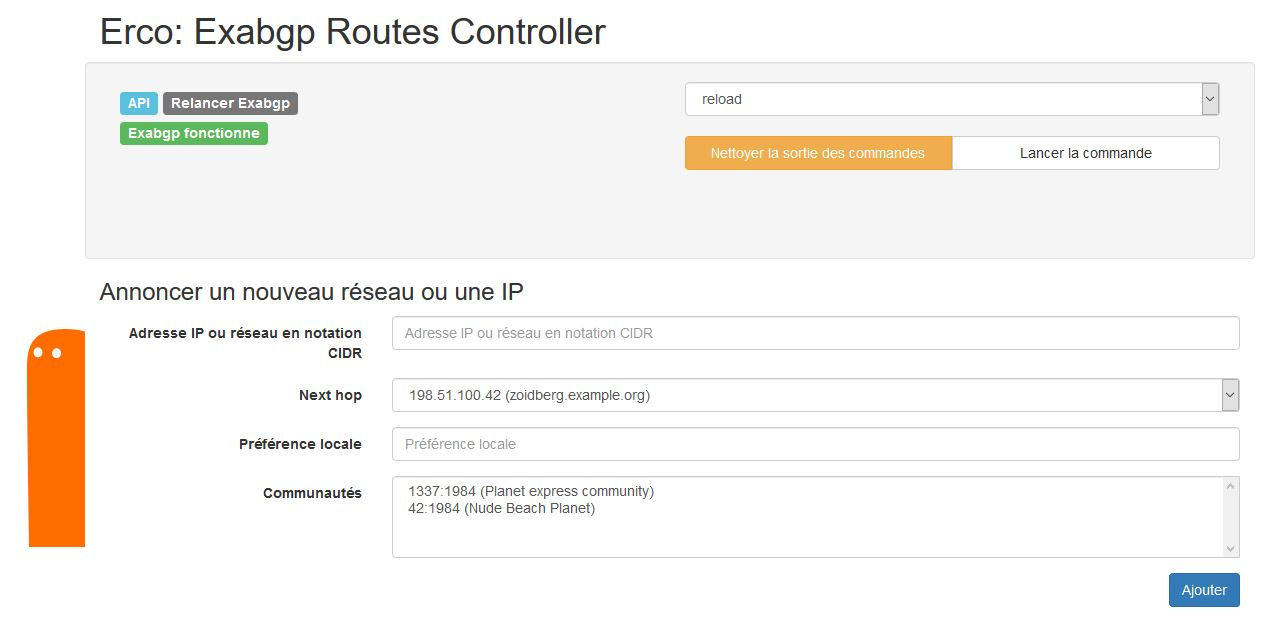
\includegraphics[scale = 0.5]{img/erco1.JPG}
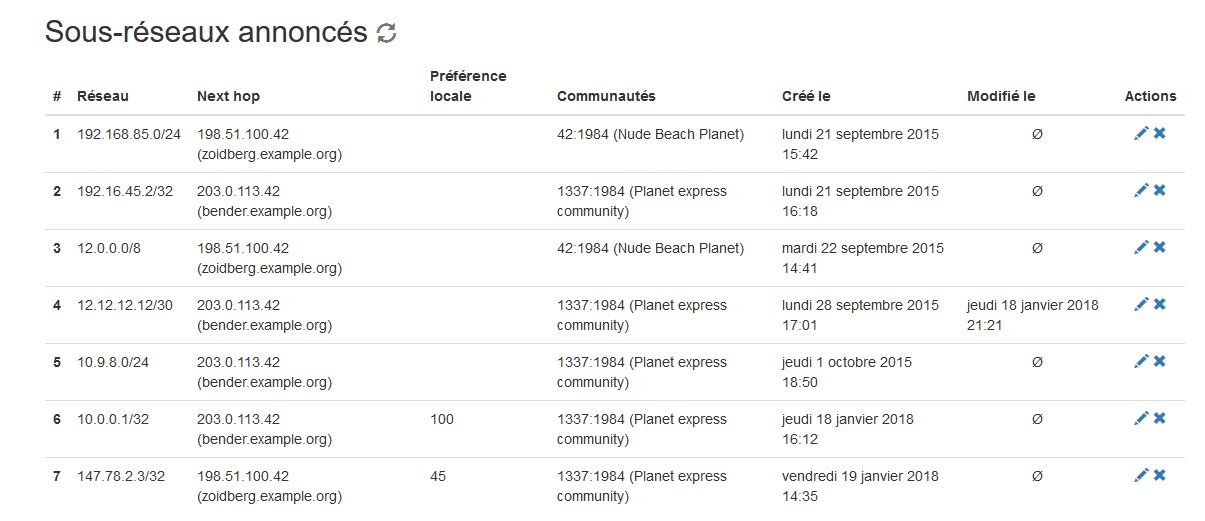
\includegraphics[scale = 0.5]{img/erco2.JPG}

\subsection{ExaBGPmon}
ExaBGPmon est une interface web sur le même principe que Erco.xyz, mais nous n'allons rien retenir de se site car il est moins intuitif et ergonomique que Erco et propose les mêmes fonctionnalités.
\\
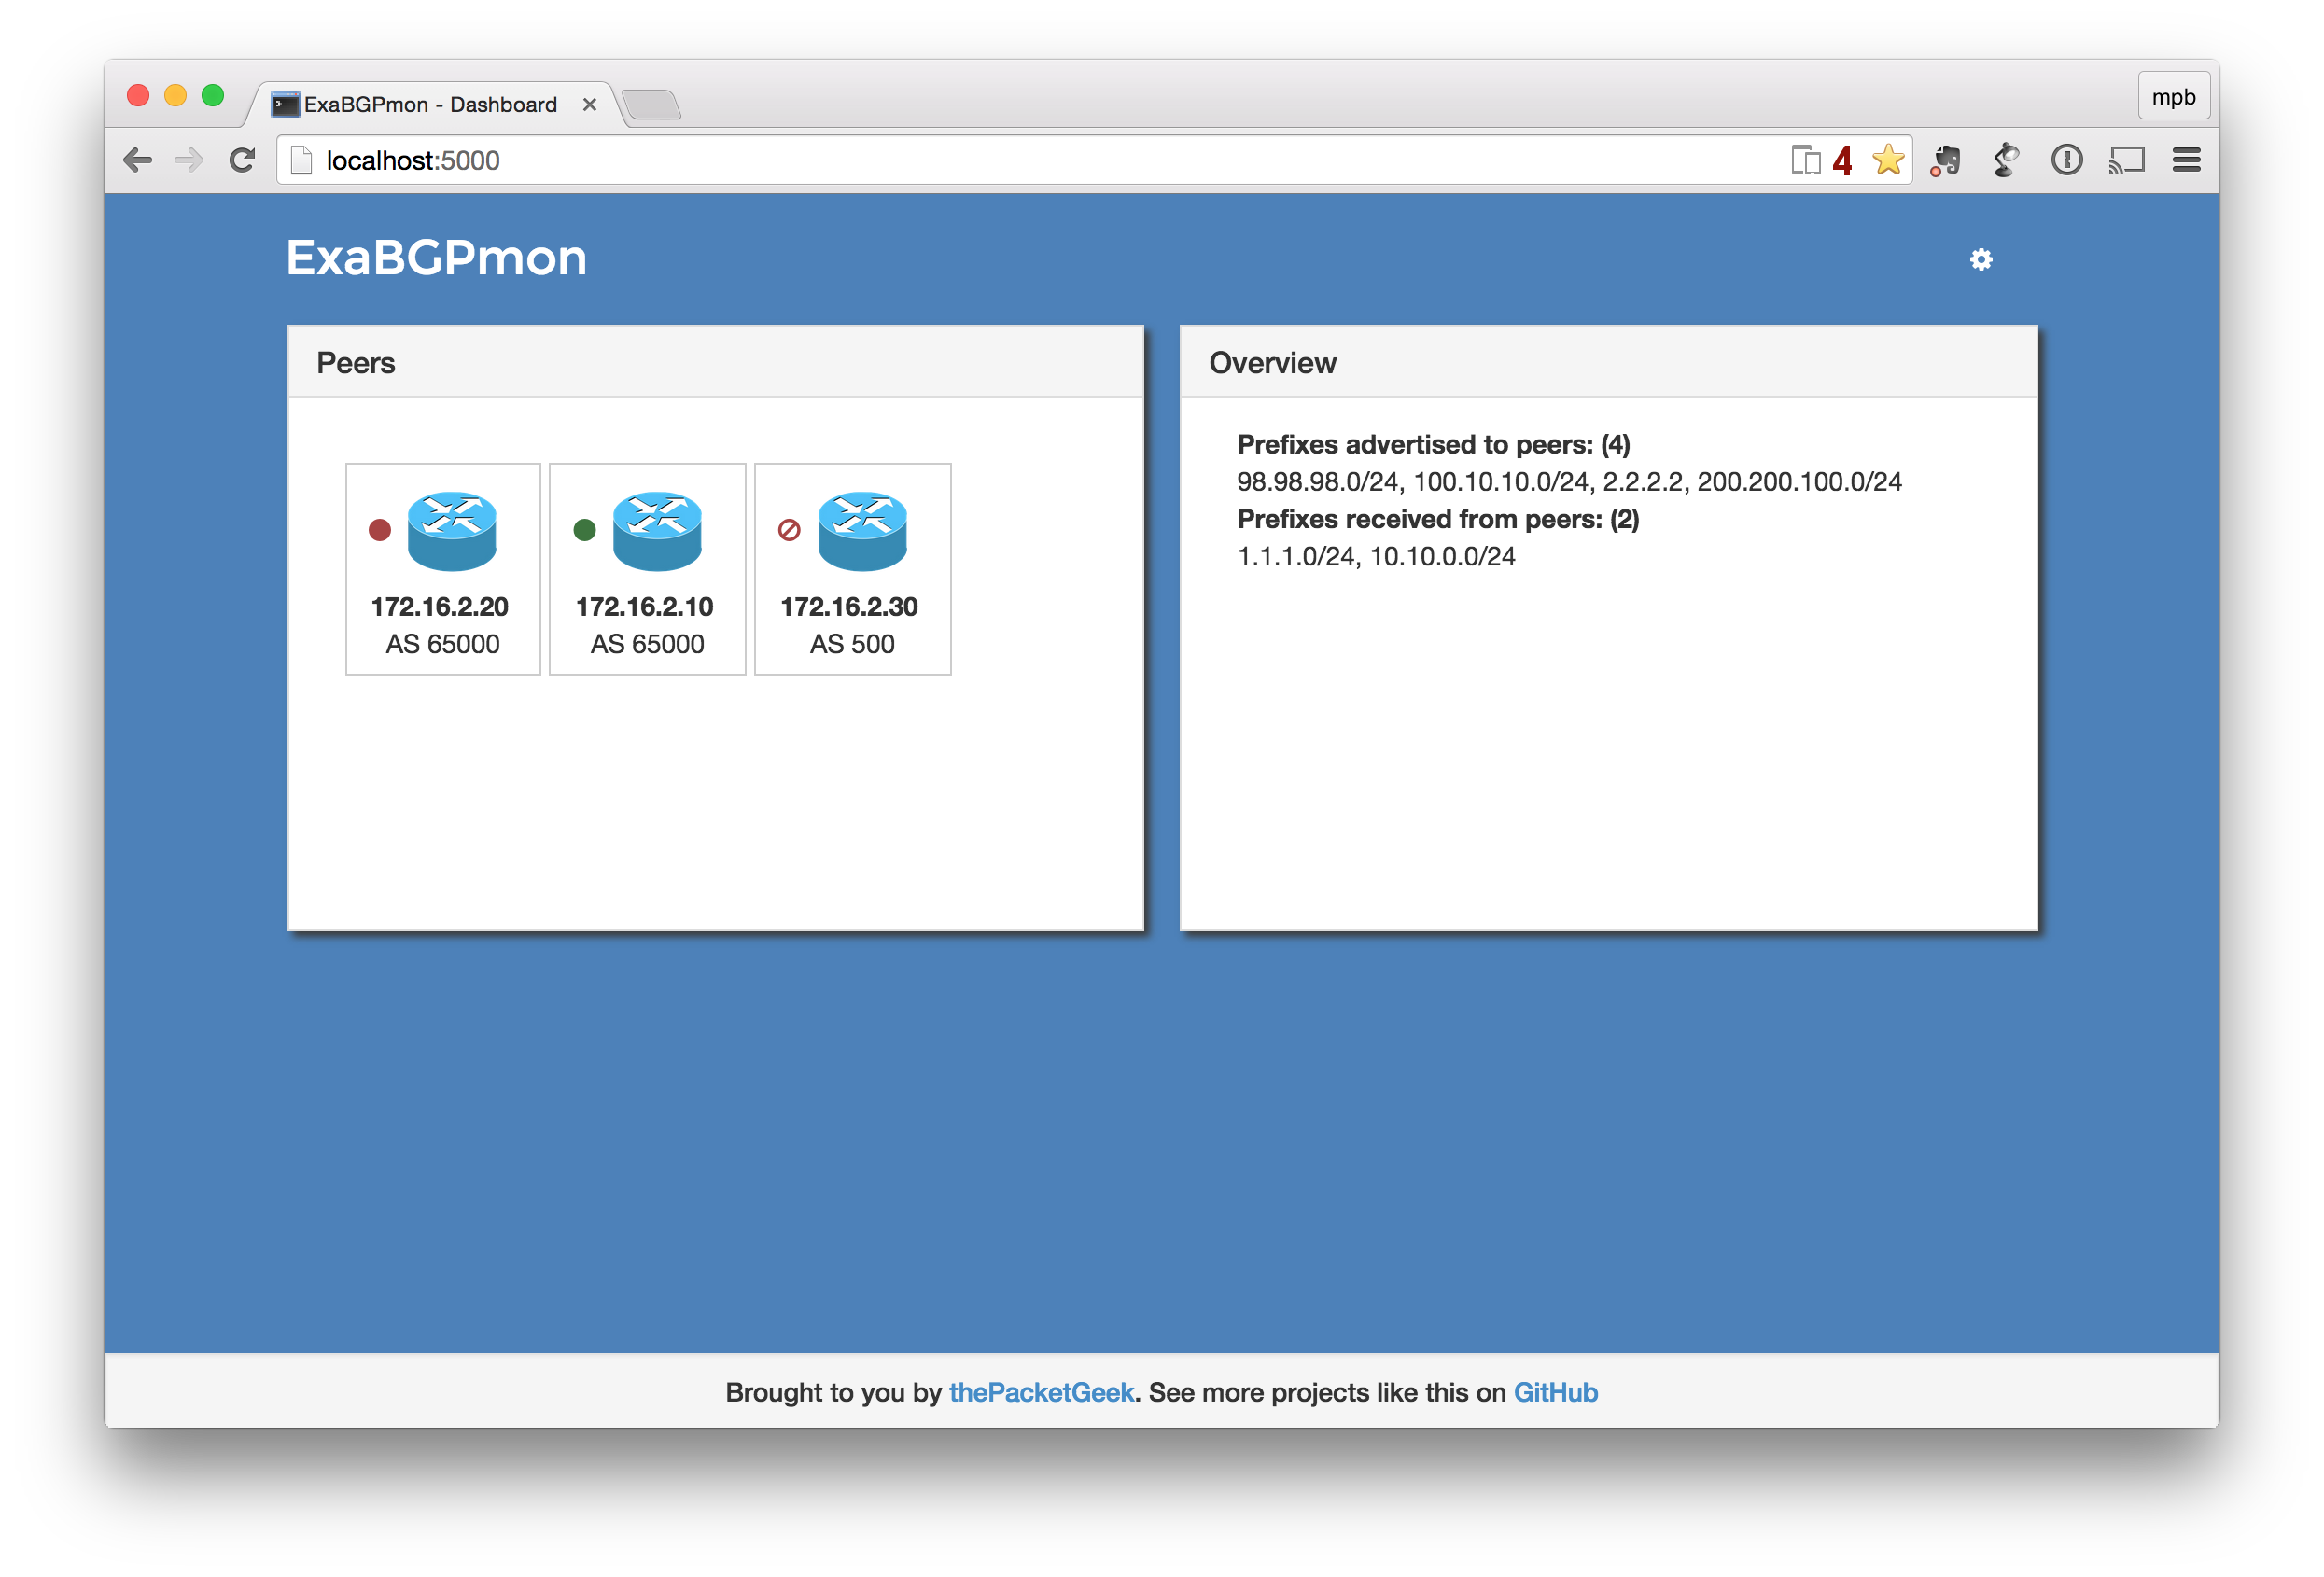
\includegraphics[scale = 0.40]{img/exabgpmon.png}


\subsection{ExaBGP}
ExaBGP est un outil open source écrit en Python qui permet d'interagir avec les réseaux BGP. Le logiciel peut injecter des routes annoncés dans les réseaux. 
ExaBGP offre un API contenant plusieurs commandes afin de manipuler les routeurs BGP. On peut aller voir la liste des commandes dans l'API d'ExaBGP : 
\\
\\
\url{https://github.com/Exa-Networks/exabgp/wiki/Controlling-ExaBGP-:-interacting-from-the-API}
\\
\\
Et apprendre à l'utiliser avec les tutos suivants:
\\
\\
\url{https://thepacketgeek.com/series/influence-routing-decisions-with-python-and-exabgp/}

\subsection{Meteor.JS \cite{Meteor.JS}}
\begin{center}

\includegraphics[height=1cm]{img/Meteor-logo.png}
\end{center}

Meteor.JS est un framework open-source javascript, Node.JS qui permet l'élaboration d'une application web de type RESTful. Elle permet de développer le client et le serveur de l'application web avec le même langage.\\
Notre client voulait une interface web développé en JavaScript de type Restful. Pour un déploiement et implémentation plus rapide de cette interface nous avons décidé d'utiliser le framework open-source Meteor.js qui réponds à ses besoins. De plus avec la possibilité d'utiliser des packages (extensions) de meteor.js nous pouvons implémenter certaines choses plus rapidement.\\
\\
Les packages utilisés sont:
\begin{itemize}
\item twbs:bootstrap
\item ian:accounts-ui-boostrap-3
\item iron:router
\end{itemize}

%client javascript RESTfull, nous plus facile package, serveur cache client.
\vspace{0.5cm}
Voici quelques liens pour pouvoir s'informer plus sur Meteor.js:
\\
\\
\url{http://meteortips.com/first-meteor-tutorial/}\\
\url{http://meteortips.com/second-meteor-tutorial/}\\
\url{http://www.meteor-tuts.com/}\\
\url{https://www.meteor.com/tutorials/react/creating-an-app}\\
Documentation: \url{http://docs.meteor.com/#/full/}


\subsection{MongoDB}\cite{MongoDB}

MongoDB est une base de données open source orientée documents qui fournit de hautes performances, une haute disponibilité, et mise à l'échelle automatique.

\section{Cahier des Charges}
Après avoir analysé les outils existants et les besoins du client, on s'est rendu compte que le client aura besoin d'une application Web de type RESTful pour pouvoir interagir avec ExaBGP.
\newline
Par conséquent, notre application Web s'appuiera sur le framework Meteor JS. 

\subsection{Besoins fonctionnels}

\subsubsection{Administrateur}
\begin{enumerate}

\item S'identifier à l'aide d'un identifiant et un mot de passe
	\begin{itemize}
		\item les informations de connexion doivent être stockées dans la base de donnée
	\end{itemize}

\item Vérifier le bon fonctionnement ExaBGP :
	\begin{itemize}
        \item Envoyer un message d'avertissement(popup)quand ExaBGP est en panne ou ne tourne pas.
	\end{itemize}

\item Annoncer une route : 
	\begin{itemize}
    	\item Envoyer une requête HTTP composé du fichier JSON au serveur ExaBGP, pour exécuter la commande 'announce route'.
		\item Annoncer un réseau ou une adresse IP à tous les BGP 'peers' afin qu'ils prennent en compte la configuration de la route entrée par l'administrateur réseau.
        \item Attribuer une communauté à une adresse IP ou à un réseau lors de l'ajout.
        \item La route sera stockée dans la base de données.
        \item En cas de succès, un message s’apparaît à l'utilisateur pour confirmer l'ajout. Dans le cas échéant, un message d'erreur est affiché à l'écran contenant le code d'erreur. 
	\end{itemize}
    
    \item Pouvoir supprimer une route :
	\begin{itemize}
		\item L'administrateur réseaux pourrait supprimer une route qui a été déjà annoncée.
        \item La route sera donc supprimée de la base de données.
        \item En cas de succès, un message s’apparaît à l'utilisateur pour confirmer la suppression. Dans le cas échéant, un message d'erreur est affiché à l'écran contenant le code d'erreur. 

	\end{itemize}
    
\item Dévier une route vers un trou noir : 
	\begin{itemize}
		\item La route sera déviée vers le trou noir selon son adresse IP source, sa destination ou bien la communauté à laquelle elle appartient.
        \item Le Next-Hop de la route sera l'interface null0.
        \item En cas de succès, un message s’apparaît à l'utilisateur pour confirmer que la route n'est plus accessible selon le préfixe définit(Source IP ou destination IP ou bien la communauté). Dans le cas échéant, un message d'erreur est affiché à l'écran contenant le code d'erreur. 

	\end{itemize}

\item Relancer ExaBGP en cas de panne :
	\begin{itemize}
		\item Un bouton permettant d'envoyer une requête HTTP au serveur ExaBGP.
        \item La requête consiste à exécuter la commande 'reload' de l'API de ExaBGP.
        \item La commande 'reload' relance la configuration d'ExaBGP sur le serveur.
        \item En cas de succès, un message de confirmation s’apparaît pour l’utilisateur. Dans le cas échéant, un message d'erreur s’apparaît portant le code d'erreur.
	\end{itemize}

\item Exécuter les différentes commandes de l'API de ExaBGP
	\begin{itemize}
        \item L'application web devrait pouvoir exécuter la totalité des commandes de L'API ExaBGP.
        \item Les commandes à exécuter seront envoyées au serveur ExaBGP en format fichier JSON.
        \item En cas d'erreur, l'application web devrait récupérer le code d'erreur de l'exécution provenant du serveur ExaBGP.
	\end{itemize}	
\end{enumerate}

\subsubsection{Administrateur et client}
\begin{enumerate}

\item Lister les routes :
	\begin{itemize}
    	\item Lorsque qu'une route est modifié, ses informations sont mises à jour dans la base de donnée
		\item L'utilisateur peut voir toutes les routes qui existent dans la base de données.
		\item Le résultat sera découpé en plusieurs pages web pour facilité la lisibilité.
	\end{itemize}   
    
\item Rechercher des routes selon leurs préfixes, (adresse IP, communauté, destination) :
	\begin{itemize}
		\item Une page web dans l'application dédiée à effectuer la recherche des routes selon leurs préfixes.
	\end{itemize}
    
\end{enumerate} 



\subsection{Besoins non fonctionnels}

%(2) mettre les scripts python et JS : une contrainte
\begin{itemize}
\item Certains packages de meteor.js
	\begin{itemize}
		\item twbs:bootstrap
        \item ian:accounts-ui-bootstrap-3
        \item iron:router
	\end{itemize}
\item Synchronisation du serveur web avec ExaBGP
\item Interface différente pour l'admin et l'utilisateur anonyme
\item Ecriture des scripts en Python et Javascript (imposé par l'utilisation de ExaBGP et Meteor)
\end{itemize}

\subsubsection{Organisation}
En effet, pour qu'on puisse commencer la phase de développement, on a besoin de virtualiser la topologie complète de réseaux et donc d'installer l'environnement technique sur nos machines (Dynamips, Nemu, et ExaBGP).
\\
\\
Concernant l'ordre de priorité, nous avons étudié les besoins du client et on en avait déduit l'ordre suivant : 
\begin{enumerate}
\item Installer l'environnement technique dans le but d'avoir une topologie virtuelle.
\item Réaliser les tâches qui concerne l'administrateur en partant de la tâche '1' jusqu'à la tâche '5'.
\item Réaliser les tâches qui concerne l'administrateur et le client dans l'ordre indiqué.
\item Enfin, réaliser la tâche '6' et '7' concernant l'administrateur.
\end{enumerate}
\section{Schéma de structure}

\begin{figure}[h]
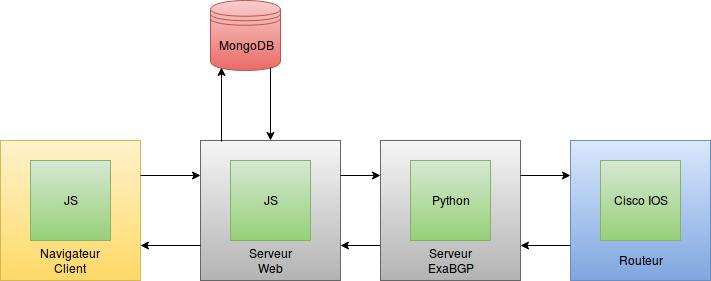
\includegraphics[scale = 0.75]{img/structure.png}
\caption{Schéma de structure}
\end{figure}


\subsection{Structure de la base de donnée}

\begin{center}
\begin{figure}[h]
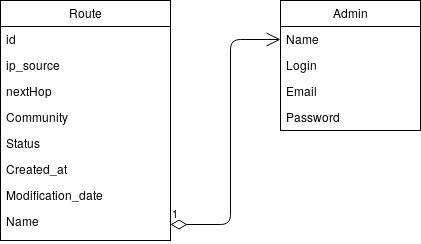
\includegraphics[scale=0.5]{img/table_mongoDB}
\caption{Uml de la base de donnée}
\end{figure}
\end{center}

La table "Route" permettra de stocker toutes les routes annoncées avec plusieurs champs spécifique:
\begin{itemize}
\item id: Une clé unique représenter par un entier positif.
\item Ip source: une adresse ip sous forme ipv4/ipv6, c'est-à-dire pour ipv4 sous la forme de quatre nombres entiers séparés par des points allant de 0.0.0.0 à 255.255.255.255. pour ipv6 8 groupes écrit en héxadécimale séparés par deux-points.
\item NextHop: une adresse ip comme ip source.
\item Community: Un tag décrivant la communauté du routeur une chaîne de caractère.
\item Status: Une chaîne de caractère qui est soit "Activate" ou "Desactivate".
\item Created at: la date de création de la route sous format <YYYY-mm-ddTHH:MM:ss> Y:année m:mois d:jour h:heure M:minute s:seconde.
\item Modification date: la date de la dernière modification sur cette route, peut être vide.
\item Name: le nom de l'administrateur qui la modifier ou ajouter représenter par une chaîne de caractère.
\end{itemize}

La table Admin permettra de stocker tout les administrateurs avec les champs suivants:
\begin{itemize}
\item Name: nom de l'administrateur représenter par une chaine de caractere.
\item Login: pseudonyme de l'administrateur représenter par une chaine de caractère.
\item Email:  une adresse mail valide de l'administrateur.
\item Password: un mot de passe.
\end{itemize}
\section{Diagramme de Gant}

\begin{table}[h]
\begin{turn}{90}
\centering
\begin{tabular}{|p{2.5cm}|*{10}{p{1.0cm}|}}

\hline
 & semaine 5: 5 fév / 9 fév & semaine 6: 12 fév / 16 fé & semaine 7: 19 fév / 23 fév & semaine 8: 26 fév / 2 mars & semaine 9 : 27 fév / 3 mars & semaine 10: 5 mars / 9 mars & semaine 11: 12 mars / 16 mars & semaine 12: 19 mars / 23 mars & semaine 13: 26 mars / 30 mars & semaine 14: 2 avr / 6 avr \\
\hline
ajouter/supprimer route & & & & & X & & & & &\\
\hline
supprimer adresse IP ou réseau & & & & X & & & & & & \\
\hline
attribution d'une communauté & & & & X & & & & & &\\
\hline
Lancer/Relancer ExaBGP & & X & & & & & & & &\\
\hline
état de ExaBGP & & X & & & & & & & &\\
& & & & & & & & & &\\
\hline
Lister les route & & X & X & & & & & & &\\
& & & & & & & & & &\\
\hline
Executer les différentes commandes d'ExaBGP & & & & & & X & X & X & &\\
\hline
Recherche IP, Route par préfixe & & & & & &  &  & X & X & X\\
\hline
connecter ExaBGP au serveur web & & X & & & & & & & &\\
\hline
Mise en place de machine virtuelle pour test & X & X & X & & & & & & &\\
\hline
\end{tabular}
\end{turn}
\end{table}

\addcontentsline{toc}{section}{Bibliographie et Références}
\bibliography{biblio}

\end{document}